\documentclass{article}

\usepackage{booktabs}
\usepackage{multirow}
\usepackage{amsmath}
\usepackage{hyperref}
\usepackage{overpic}
\usepackage{amssymb}
\usepackage{graphicx}

\usepackage[accepted]{dlaiml2026}

% Generated by scripts/report_numbers.py. Do not edit by hand.
% Every number quoted in the report is defined here and nowhere else.
\newcommand{\NSeeds}{3}
\newcommand{\NEpochs}{20}
\newcommand{\BatchSize}{128}
\newcommand{\BinSize}{10}
\newcommand{\NBins}{124}
\newcommand{\NTest}{10\,000}
\newcommand{\BaseGreyErr}{14.71}
\newcommand{\BaseGreySat}{0.0}
\newcommand{\BaseGreySpread}{0.0}
\newcommand{\BaseMeanErr}{14.64}
\newcommand{\BaseMeanSat}{39.0}
\newcommand{\BaseMeanSpread}{0.0}
\newcommand{\LtwoErr}{12.44~[12.42, 12.47]}
\newcommand{\LtwoSat}{62.0~[61.1, 63.1]}
\newcommand{\LtwoSpread}{53.8~[53.2, 54.4]}
\newcommand{\LtwoWithin}{70.6~[70.5, 70.7]}
\newcommand{\ClsModeT}{0.02}
\newcommand{\ClsModeErr}{13.61~[13.60, 13.63]}
\newcommand{\ClsModeSat}{62.9~[62.8, 63.0]}
\newcommand{\ClsModeSpread}{57.1~[56.7, 57.7]}
\newcommand{\ClsBestT}{0.65}
\newcommand{\ClsBestErr}{12.32~[12.32, 12.33]}
\newcommand{\ClsBestSat}{57.6~[57.3, 57.8]}
\newcommand{\ClsBestSpread}{50.5~[50.2, 50.9]}
\newcommand{\ClsMeanT}{1}
\newcommand{\ClsMeanErr}{12.43~[12.41, 12.46]}
\newcommand{\ClsMeanSat}{63.9~[63.7, 64.3]}
\newcommand{\ClsMeanSpread}{53.9~[53.5, 54.3]}
\newcommand{\MechSame}{3.11~[3.07, 3.15]}
\newcommand{\MechCross}{3.11~[3.08, 3.14]}
\newcommand{\MechMode}{6.78~[6.64, 6.96]}
\newcommand{\MechTruth}{12.49~[12.47, 12.52]}
\newcommand{\MechCorr}{0.896}
\newcommand{\PerClassInstances}{+0.36}
\newcommand{\PerClassPixels}{+0.02}
\newcommand{\MechRatio}{4.0}


\dlaititlerunning{Mean or Mode}

\begin{document}

\twocolumn[
\dlaititle{Mean or Mode: What the Loss Chooses When Colour Is Ambiguous}

\begin{center}\today\end{center}

\begin{dlaiauthorlist}
\dlaiauthor{Stefano Solazzo}{}
\end{dlaiauthorlist}

\dlaicorrespondingauthor{Stefano Solazzo}{solazzo.1911897@studenti.uniroma1.it}

\vskip 0.3in
]

\printAffiliationsAndNotice{}

\begin{abstract}
%
Colourising a greyscale photograph has no single correct answer: a grey car is
consistent with red, blue or white, and under a squared error the optimal
prediction is then the mean of the plausible colours, which is close to grey.
Two colourisers are trained on CIFAR-10 with everything but the loss held fixed,
the second reading its predicted distribution at a temperature that interpolates
between that distribution's mean and its mode. Sweeping it traces a frontier on
which accuracy and colour variety cannot both be maximised. At temperature one
the classification network reproduces the squared error network pixel by pixel,
\MechSameBare{} apart against the \MechTruthBare{} separating either from the
truth, and does so across independent seeds: the desaturation is a property of the question
the loss asks, not of a model or a run.
%
\end{abstract}

% ------------------------------------------------------------------------------
\section{Introduction}

Given the lightness of a photograph, what colour was it? For many pixels the
question has no answer: a greyscale car constrains its colour hardly at all, a
greyscale frog constrains it a great deal. What exists is not a function from
lightness to colour but a conditional distribution $p(a,b \mid L)$.

A network emits one colour per pixel, so something must collapse that
distribution, and the loss decides what. Let $\mu = \mathbb{E}[Y \mid X = x]$.
Adding and subtracting $\mu$ inside the squared error and expanding gives
%
\begin{equation}\label{eq:mean}
\mathbb{E}\big[\lVert \hat{y} - Y \rVert^2\big]
  = \lVert \hat{y} - \mu \rVert^2 + \operatorname{Var}(Y \mid X = x)\,,
\end{equation}
%
since the cross term contains $\mathbb{E}[\mu - Y] = 0$. The second term is
independent of the prediction, so the minimiser is $\hat{y} = \mu$
\cite{bishop2006pattern}: the model produces not a plausible colour but the
average of the plausible ones, and the average of red, blue and white is a
barely tinted grey.

% ------------------------------------------------------------------------------
\section{Related work}

Posing colourisation as classification over quantised $ab$ bins, and decoding
with an annealed mean, is due to Zhang et al.~\cite{zhang2016colorful}; Larsson
et al.~\cite{larsson2016learning} independently predicted per-pixel colour
histograms. That a squared error averages ambiguous targets is likewise
established~\cite{mathieu2016beyond}. Neither is claimed as new. What is added
is a controlled measurement: everything but the loss is held fixed, the frontier
is traced by one knob rather than two tuned systems, and the networks are
compared against each other pixel by pixel. Three departures
from~\cite{zhang2016colorful} follow: their class rebalancing is a second
mechanism for raising vividness and would confound the trade measured here, so
the cross-entropy is left plain; their fixed 313-bin grid becomes the same
\BinSize{}-unit grid cut to the cells the data visits; and CIFAR-10 replaces
ImageNet.

% ------------------------------------------------------------------------------
\section{Method}

Work is in CIE Lab, which separates the lightness the network is given from the
chroma it must guess and in which euclidean distance approximates perceived
colour difference. The network receives $L$ and predicts $(a,b)$ everywhere.

\paragraph*{Architecture.} Six blocks of $3\times3$ convolution, batch
normalisation~\cite{ioffe2015batchnorm} and ReLU at $64$ channels, dilations
$1,1,2,4,8,1$~\cite{yu2016dilated}, then a $1\times1$ convolution to the output.
Dilation rather than striding keeps full resolution and gives a receptive field
of $35$ pixels, wider than the image, so residual uncertainty is ambiguity in
the data and not myopia. Everything up to it is shared; the first model
minimises the squared error on $(a,b)$, the second quantises the $ab$ plane into
\BinSize{}-unit cells, keeps the \NBins{} holding \BinCoverage{}\% of the
training pixels, and minimises the cross-entropy over them.

\paragraph*{Readout.} With bin centres $c_k$ and probabilities $p_k$,
%
\begin{equation}\label{eq:annealed}
\hat{y}(T) = \sum_k \frac{\exp(\log p_k / T)}{\sum_j \exp(\log p_j / T)}\, c_k \,,
\end{equation}
%
the distribution's mean at $T=1$, which is what Equation~\eqref{eq:mean}
predicts the squared error model produces, and its mode as $T \to 0$.

\paragraph*{Metrics and protocol.} Colour error is the mean euclidean distance
to the truth in $ab$; vividness is mean chroma against the truth's own. Since a
model painting every pixel the same beige already scores \BaseMeanSat{}\% on it,
variety, the mean distance from the model's own average output and zero for any
constant prediction, sits beside it.
\NSeeds{} seeds, \NEpochs{} epochs, batch \BatchSize{},
AdamW~\cite{loshchilov2019adamw} with a one-cycle
schedule~\cite{smith2019onecycle}, in PyTorch~\cite{paszke2019pytorch} on a
laptop GPU. All numbers are on the \NTest{} held-out test images of
CIFAR-10~\cite{krizhevsky2009cifar}, brackets giving the range over seeds;
labels are never shown to the colourisers.
Code:
\url{https://github.com/solazzo1911897-collab/colorization-mean-vs-mode}.

% ------------------------------------------------------------------------------
\section{Results}

\begin{figure}[!t]
    \centering
    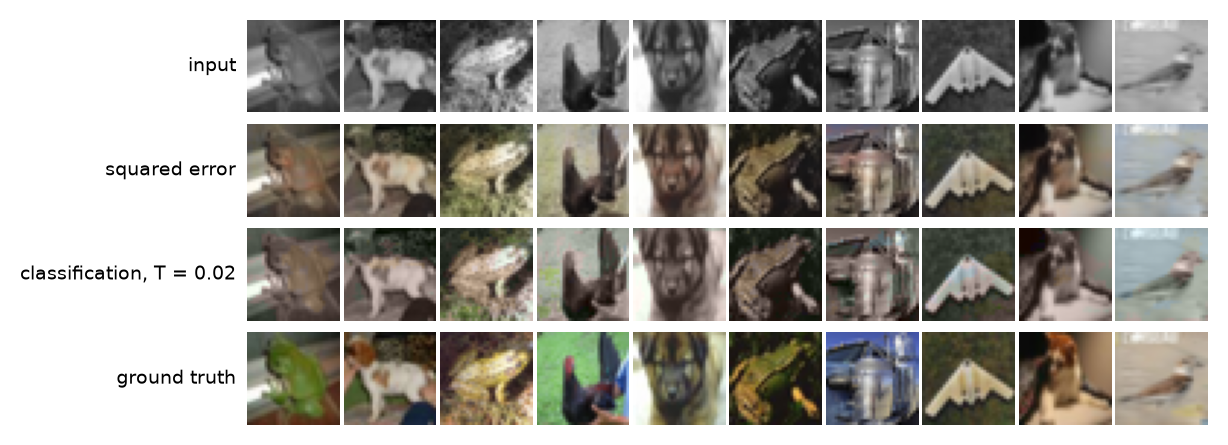
\includegraphics[width=0.88\linewidth]{../figures/fig1_qualitative.png}
    \caption{The two losses on the same test images, the classification model
    read at its mode. Both are muted against the truth, and muted in nearly the
    same way. One seed of each.}
    \label{fig:qualitative}
\end{figure}

\paragraph*{Baselines and the cost of the mean.} Grey everywhere gives
\BaseGreyErr{} error; the average training colour gives \BaseMeanErr{} at
\BaseMeanSat{}\% vividness and \BaseMeanSpread{}\% variety. The squared error
model reaches \LtwoErr{} at
\LtwoSat{}\% vividness and \LtwoSpread{}\% variety, beating both
(Figure~\ref{fig:qualitative}).

\paragraph*{The frontier.} Sweeping $T$ (Figure~\ref{fig:frontier}) turns one
prediction into a curve, and the squared error model sits on it: at
$T=\ClsMeanT{}$ the classification model gives \ClsMeanErr{} and
\ClsMeanSpread{}\% variety against \LtwoErr{} and \LtwoSpread{}\%. Toward the
mode variety rises and accuracy falls, from \ClsBestSpread{}\% at \ClsBestErr{}
($T=\ClsBestT{}$, lowest error) to \ClsModeSpread{}\% at \ClsModeErr{}. Neither
end wins on both axes, and the squared error model cannot move along the curve
at all. The range is narrow: even at the mode only \ClsModeSat{}\% of the
truth's vividness is kept against \LtwoSat{}\%, the conditional distribution
being concentrated enough here that its mean and its mode nearly coincide, so
the readout alone cannot close the gap.

\begin{figure}[!t]
    \centering
    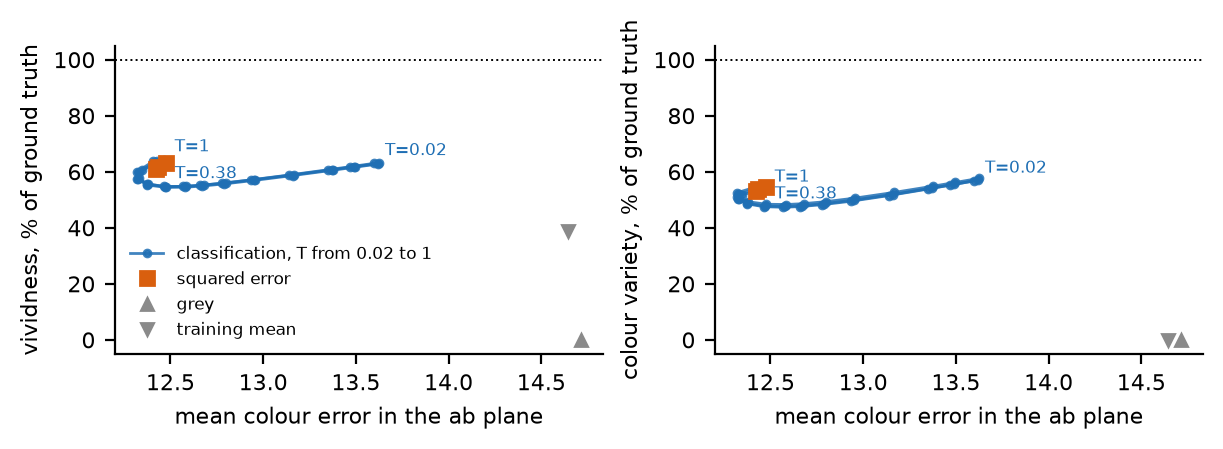
\includegraphics[width=0.88\linewidth]{../figures/fig2_frontier.png}
    \caption{Accuracy against vividness (left) and variety (right) as the
    readout temperature is swept; all \NSeeds{} seeds drawn. The constant
    baseline sits at \BaseMeanSat{}\% vividness and zero variety.}
    \label{fig:frontier}
\end{figure}

\paragraph*{The two models are one model.} Equation~\eqref{eq:mean} predicts the
squared error output should coincide with the expectation of the classification
model's distribution, and it does: \MechSame{} in $ab$ units between them
against \MechTruth{} between either and the truth, a factor of \MechRatio{};
against that model's mode it is \MechMode{}
(Figure~\ref{fig:mechanism}). The scale that makes that small is not the
distance to the truth but the run-to-run floor: two squared error models
differing only in seed are \WithinLtwo{} apart, two classification models
\WithinCls{}, so changing the loss moves the output about as far as changing
the initialisation. Pairing across seeds changes nothing, \MechCross{}.

\paragraph*{A prediction that failed.} The desaturation was expected to be worst
where colour is least predictable, yet grouped by CIFAR-10 class the correlation
with the squared error model's vividness is \PerClassInstances{} between
instances and \PerClassPixels{} over all pixels, and per pixel against the
classification model's own predictive entropy \EntropyCorrLtwo{}: no relation in
the predicted direction, and one confound behind both (appendix).

\paragraph*{Discussion.} That the two models agree is what
Equation~\eqref{eq:mean} predicts, so this is a confirmation rather than a
surprise. What it adds is that the agreement survives finite data and runs
sharing nothing but the loss, locating the desaturation in the objective, not in
any model. Vividness must therefore come from the readout or from reweighting
rare colours, not from the loss.

% ------------------------------------------------------------------------------
\section*{Statement on the use of AI}

Anthropic's Claude was used as an assistive tool throughout this
project. It supported the refinement of the experimental methodology,
assisted in extending and debugging the codebase, and aided in source
verification and bibliographic assembly. It was also employed to polish,
format, and synthesize drafts into the final report.

The Lab conversion was validated against published sRGB primaries, all
citations were cross-checked at source, and all numerical values were
derived directly from run logs. Failed predictions (e.g., Section~4)
have been retained as observed.


\bibliography{references.bib}
\bibliographystyle{dlaiml2026}

\section*{Appendix}

\paragraph*{Limitations.} The resolution, at which colour ambiguity carries no
texture component; a single dataset family; the absence of any perceptual
evaluation, which for colourisation is what ultimately matters and requires
human judgement rather than a distance in Lab; the temperature reported as
lowest-error is read off the test sweep rather than a held-out split, so it is
a description of the curve and not a tuned setting; and class rebalancing,
excluded by design, whose contribution to vividness is the obvious next
measurement.

\paragraph*{The sweep doubles back.} Both vividness and variety are U-shaped in
$T$ with a minimum near $T = 0.3$, where the softmax is flat enough to pull the
readout toward the centroid of the bin grid but not flat enough to reach it, so
the curve of Figure~\ref{fig:frontier} folds rather than tracing a single
monotone trade.

\paragraph*{The grid is not the ceiling.} Dropping the cells the training set
barely visits is the obvious thing to suspect when a colouriser comes out
desaturated. It is not the cause here. Quantising the ground truth itself to
the \NBins{} kept centres and scoring it as though it were a prediction gives
\QuantErr{} colour error at \QuantSat{}\% vividness, slightly above the truth's
own rather than below it, since a near-grey pixel is moved out to a cell centre;
\BinCoverage{}\% of test pixels fall inside a cell that was kept. The integer
lookup that replaces the distance matrix when encoding a pixel agrees with the
exact nearest centre \LutAgree{}\% of the time and lands \LutExcess{}\% further
away when it does not.

\paragraph*{Ambiguity measured per pixel.} The failed prediction of Section 4
has a per-pixel form: the pixels where the classification model's predicted
distribution is widest should be the desaturated ones. Sorted into
\EntropyBuckets{} equal-count buckets of predictive entropy
(Figure~\ref{fig:entropy}) the correlation with vividness is
\EntropyCorrLtwo{} for the squared error model and \EntropyCorrCls{} for the
classification model, and the curve is not monotone in either. The measure
carries the same defect as the per-class one, and it is visible here: the true
chroma of a bucket grows by a factor of \EntropyChromaRatio{} from the lowest
entropy to the highest, so the denominator of the ratio moves with the quantity
being tested. Whether desaturation tracks ambiguity is a question neither
measurement answers.

\begin{figure}[h]
    \centering
    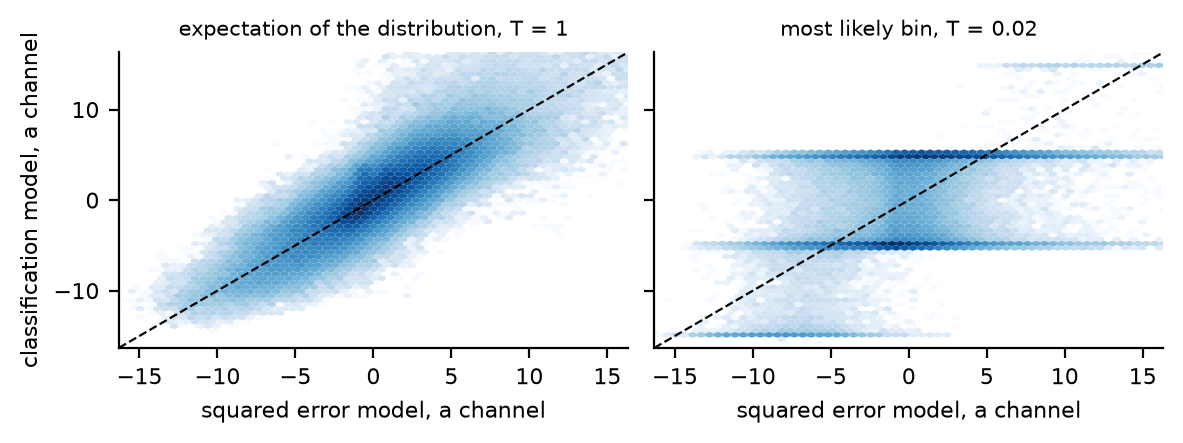
\includegraphics[width=0.99\linewidth]{../figures/fig4_mechanism.png}
    \caption{Squared error output against the classification readout, per pixel,
    on the $a$ channel, for one seed of each. Left, the expectation of its
    distribution, which agrees along the diagonal; right, its most likely bin,
    where the correspondence is gone and the discrete bin centres band the plot.
    The distances quoted in the text average over all \NSeeds{} seeds of each
    loss.}
    \label{fig:mechanism}
\end{figure}

\begin{figure}[h]
    \centering
    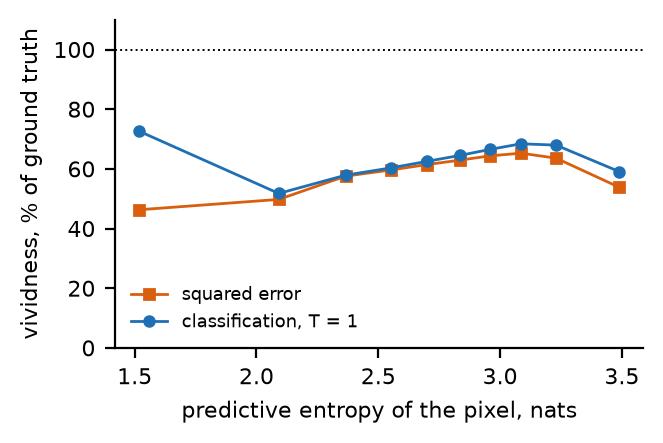
\includegraphics[width=0.72\linewidth]{../figures/fig6_entropy.png}
    \caption{Vividness against the classification model's own predictive
    entropy, one point per equal-count bucket of test pixels. The predicted
    relation is a fall to the right; neither model shows one.}
    \label{fig:entropy}
\end{figure}


\begin{figure}[h]
    \centering
    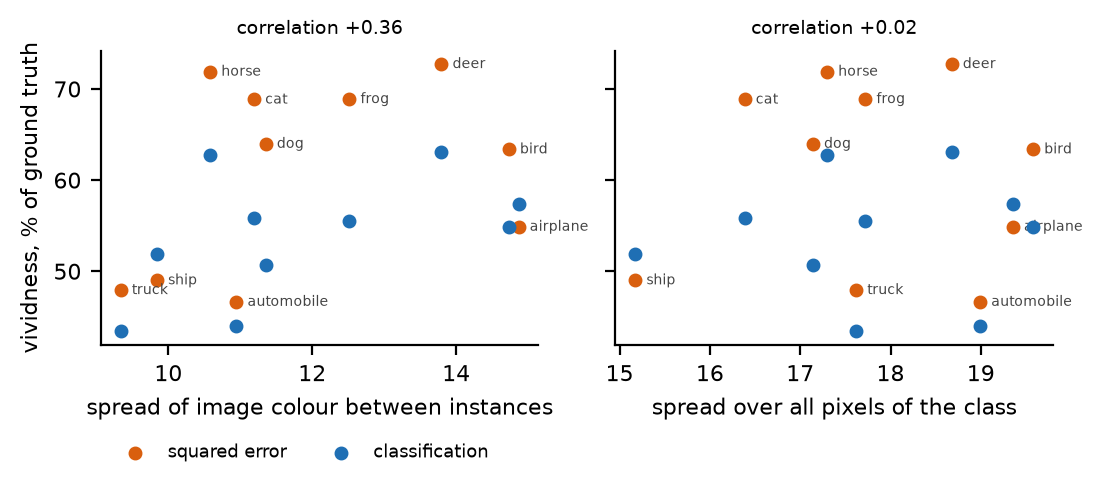
\includegraphics[width=0.99\linewidth]{../figures/fig3_per_class.png}
    \caption{Vividness against two measures of how ambiguous the colour of a
    CIFAR-10 class is. Neither shows the predicted relation. Vividness is
    reported as a ratio to each class's own ground truth, so classes dominated
    by large saturated regions of sky or sea carry a high denominator whatever
    their ambiguity, and the measure conflates the two. Kept because the
    prediction was made before the measurement.}
    \label{fig:perclass}
\end{figure}

\begin{figure}[h]
    \centering
    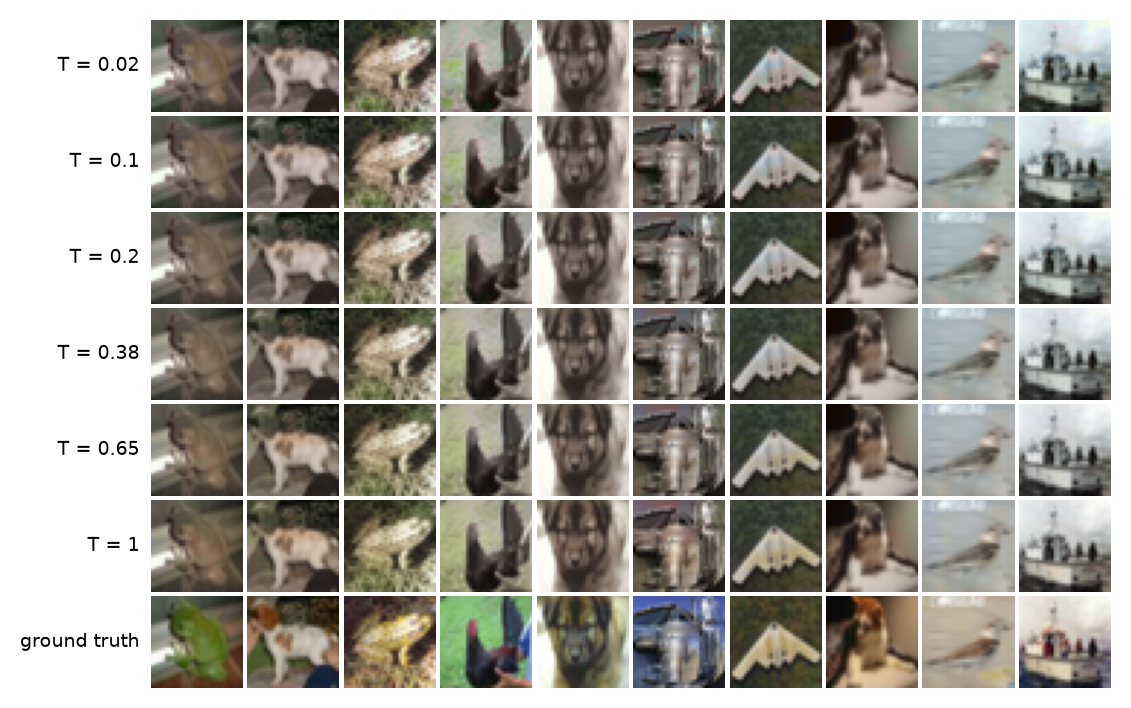
\includegraphics[width=0.99\linewidth]{../figures/fig5_temperature.png}
    \caption{The same images decoded at increasing temperature, from the most
    likely colour to the mean of the distribution.}
    \label{fig:temperature}
\end{figure}

\end{document}
